\appendix
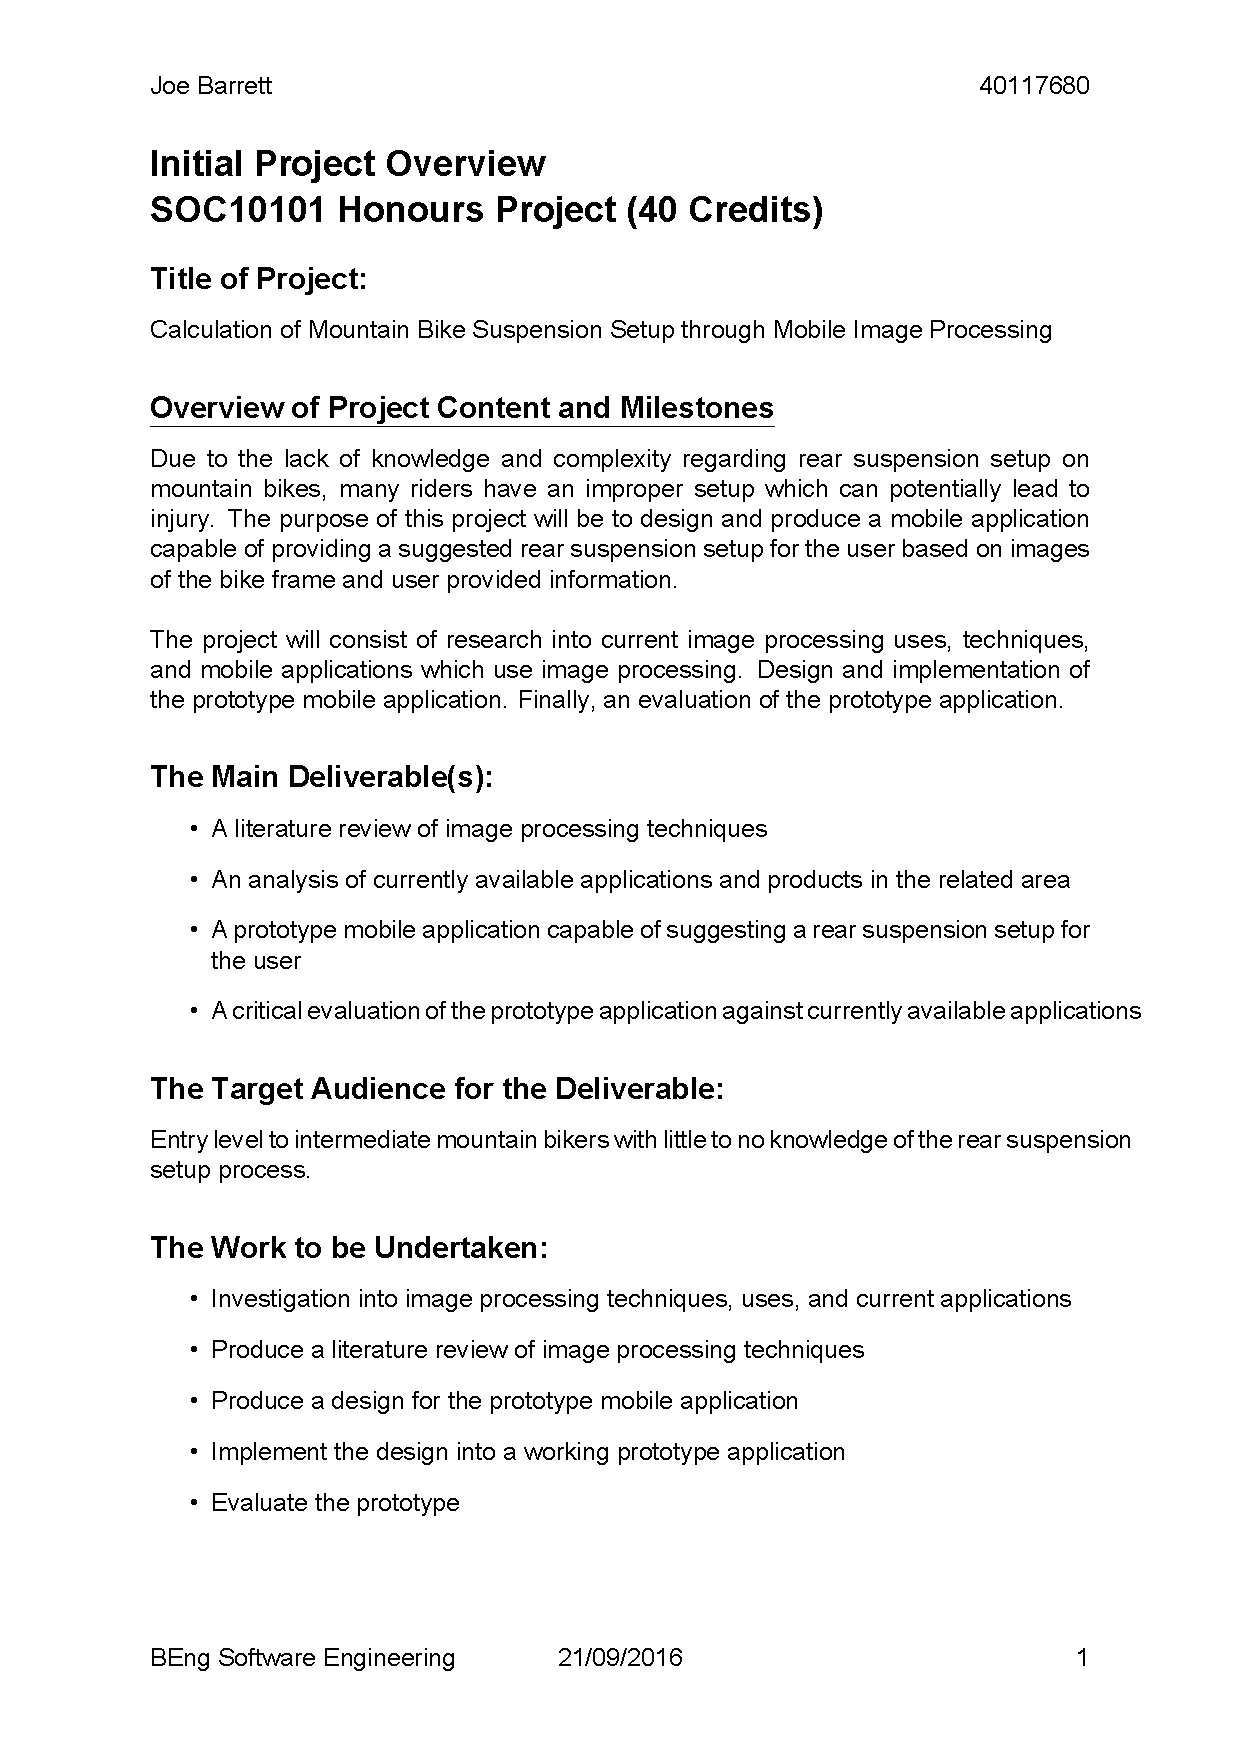
\includepdf[scale=0.9,
			pages=1,
			pagecommand=\section{Initial Project Overview},
			offset=0 -1cm]{../ipo/ipo.pdf}
\includepdf[scale=0.9,
			pages=2-,
			pagecommand={}]{../ipo/ipo.pdf}
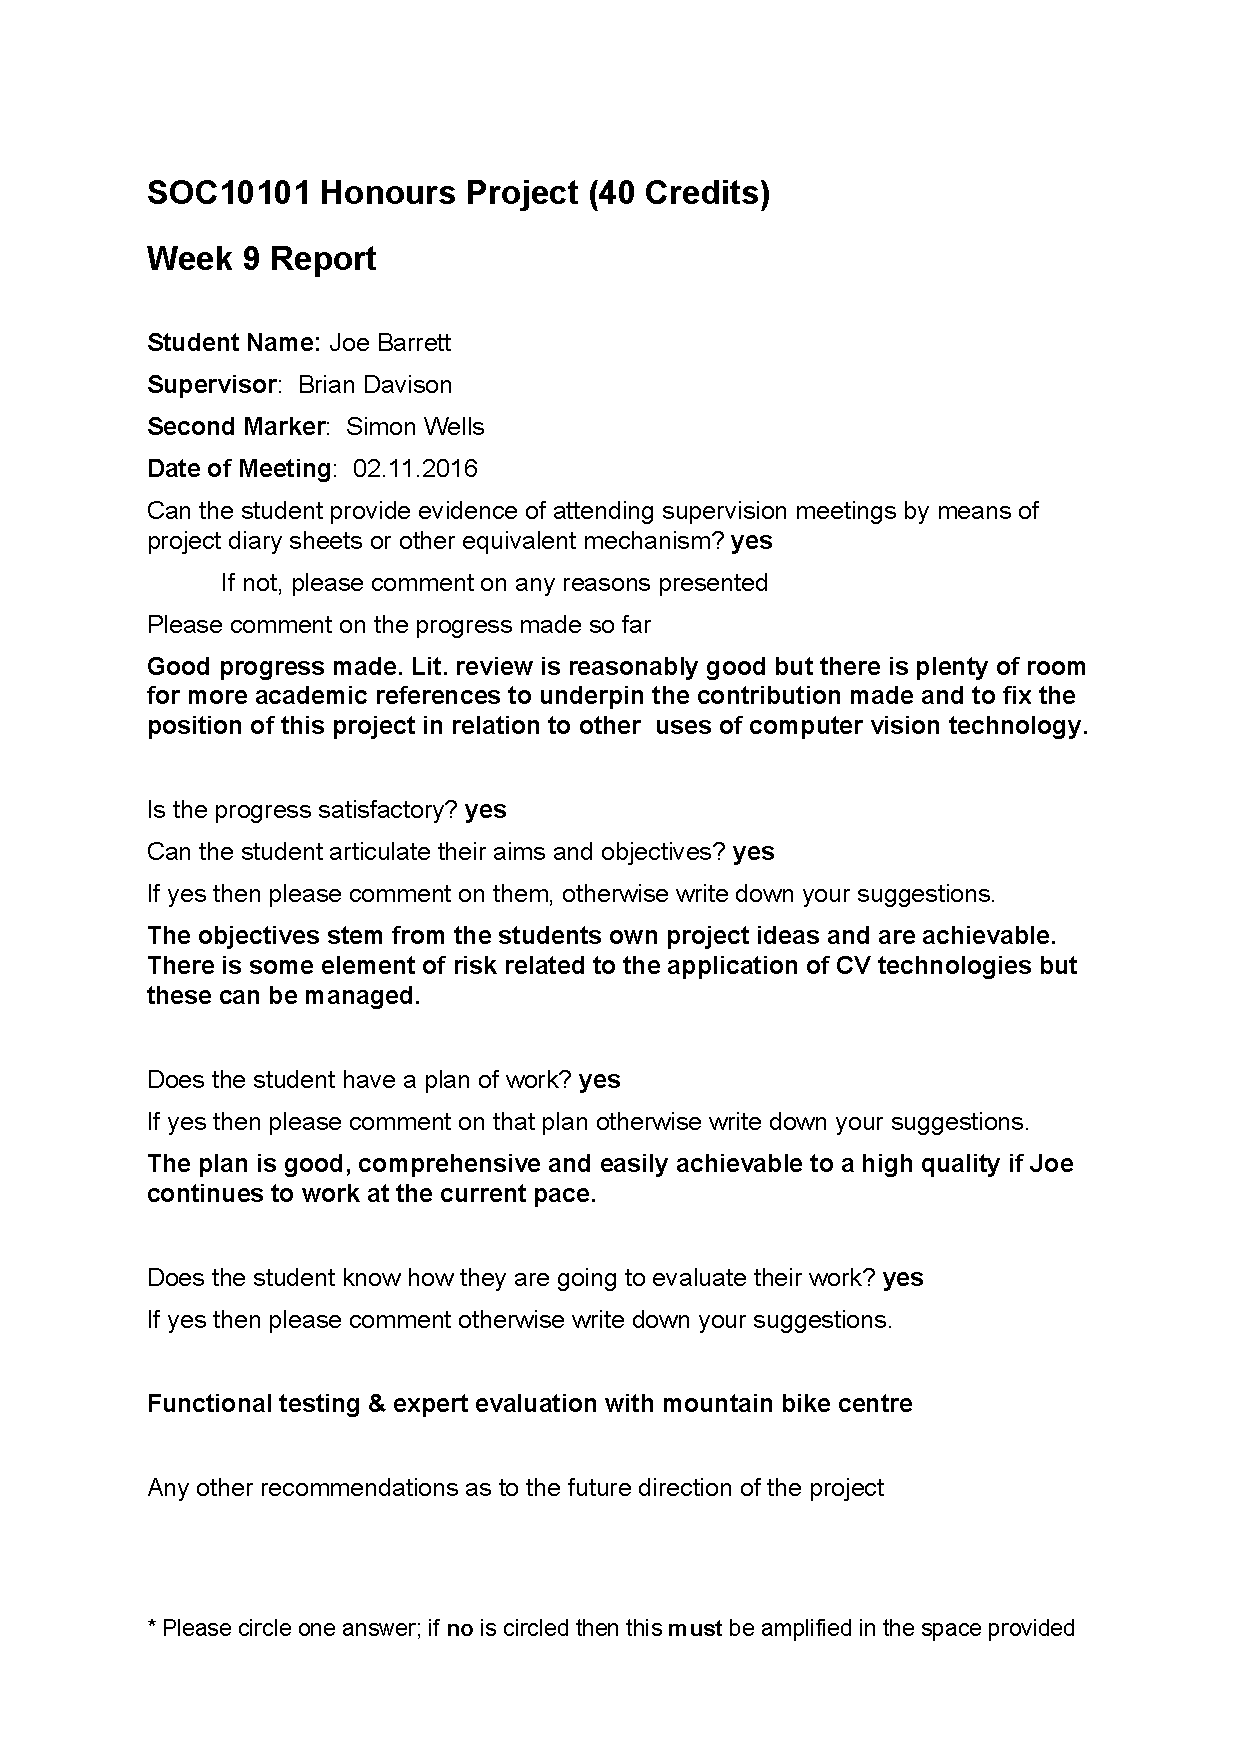
\includepdf[scale=0.9,
			pages=1,
			pagecommand=\section{Week 9 Report}]{../week_9_report.pdf}
\includepdf[scale=0.9,
			pages=2-,
			pagecommand={}]{../week_9_report.pdf}
\clearpage
\thispagestyle{empty}
\newgeometry{margin=1cm}
\begin{landscape}
	\section{Android Experiments}\label{app:android_experiments}
		\subsection{Table of Android Experiments}
		\begin{table}[h!]
			\centering
			\label{tab:android_experiments}
			\begin{tabular}{|l|p{0.4\textwidth}|l|p{0.4\textwidth}|r|r|}
				\hline
				\bfseries Experiment&\bfseries Purpose&\bfseries Functional&\bfseries Issues&\bfseries Files&\bfseries LOC\\
				\hline
				Hello CV&
				\begin{itemize}[noitemsep,topsep=0pt,parsep=0pt]
					\item{Introduction to the android OpenCV library}
					\item{Displays camera feed with fps}
				\end{itemize}&
				Yes&
				\begin{itemize}[noitemsep,topsep=0pt,parsep=0pt]
					\item{Not fullscreen}
					\item{Incorrect orientation}
				\end{itemize}&
				2&
				101\\
				\hline
				15Tile&
				\begin{itemize}[noitemsep,topsep=0pt,parsep=0pt]
					\item{Sliding tile game}
					\item{Uses camera feed as puzzle}
				\end{itemize}&
				Yes&
				\begin{itemize}[noitemsep,topsep=0pt,parsep=0pt]
					\item{Not fullscreen}
				\end{itemize}&
				3&
				492\\
				\hline
				Blob Detection&
				\begin{itemize}[noitemsep,topsep=0pt,parsep=0pt]
					\item{Demonstrates blob detection}
					\item{Runs blob detection on tapped area from camera}
				\end{itemize}&
				No&
				\begin{itemize}[noitemsep,topsep=0pt,parsep=0pt]
					\item{Crash on screen tap}
				\end{itemize}&
				3&
				311\\
				\hline
				Face Detection&
				\begin{itemize}[noitemsep,topsep=0pt,parsep=0pt]
					\item{Detects faces in camera view}
					\item{Puts boundary around detected faces}
				\end{itemize}&
				No&
				\begin{itemize}[noitemsep,topsep=0pt,parsep=0pt]
					\item{Crash on load}
				\end{itemize}&
				3&
				279\\
				\hline
			\end{tabular}
		\end{table}
	\end{landscape}
\restoregeometry
\subsection{Hello CV}
	\inputminted[breaklines,
					linenos,
					frame=lines,
					fontsize=\footnotesize]{java}{../code/android/hello_cv/MainActivity.java}
	\subsection{15tile}
	\inputminted[breaklines,
					linenos,
					frame=lines,
					fontsize=\footnotesize]{java}{../code/android/15tile/MainActivity.java}
	\inputminted[breaklines,
					linenos,
					frame=lines,
					fontsize=\footnotesize]{java}{../code/android/15tile/PuzzleProcessor.java}
	\subsection{BLOB Analysis}
	\inputminted[breaklines,
					linenos,
					frame=lines,
					fontsize=\footnotesize]{java}{../code/android/blob_analysis/ColorBlobDetectionActivity.java}
	\inputminted[breaklines,
					linenos,
					frame=lines,
					fontsize=\footnotesize]{java}{../code/android/blob_analysis/ColorBlobDetector.java}
	\subsection{Face Detection}
	\inputminted[breaklines,
					linenos,
					frame=lines,
					fontsize=\footnotesize]{java}{../code/android/face_recognition/DetectionBasedTracker.java}
	\inputminted[breaklines,
					linenos,
					frame=lines,
					fontsize=\footnotesize]{java}{../code/android/face_recognition/FrActivity.java}
	\clearpage
		\thispagestyle{empty}
		\newgeometry{margin=1cm}
		\begin{landscape}
			\section{Python Experiments}\label{app:python_experiments}
			\subsection{Table of Python Experiments}
			\begin{table}[h!]
				\centering
				\label{tab:python_experiments}
				\begin{tabular}{|l|p{0.4\textwidth}|l|p{0.4\textwidth}|r|r|}
					\hline
					\bfseries Experiment&\bfseries Purpose&\bfseries Functional&\bfseries Issues&\bfseries Files&\bfseries LOC\\
					\hline
					Find Game&
					\begin{itemize}[noitemsep,topsep=0pt,parsep=0pt]
						\item{Identify red game cartridge out of 3}
						\item{Displays boundary around correct part of image}
					\end{itemize}&
					Yes&
					N/A&
					1&
					18\\
					\hline
					Threshold Methods&
					\begin{itemize}[noitemsep,topsep=0pt,parsep=0pt]
						\item{Demonstrates various thresholding methods on an image}
						\item{Original image text unreadable but clear after techniques are applied}
					\end{itemize}&
					Yes&
					N/A&
					1&
					14\\
					\hline
					Image Operations&
					\begin{itemize}[noitemsep,topsep=0pt,parsep=0pt]
						\item{Moves parts of an image to other locations using arrays}
						\item{Demonstrates how pixel data is stored}
					\end{itemize}&
					Yes&
					N/A&
					1&
					15\\
					\hline
					Distance to Camera&
					\begin{itemize}[noitemsep,topsep=0pt,parsep=0pt]
						\item{Calculates distance to the camera from an identified object}
						\item{Displays various distances using 3 images}
					\end{itemize}&
					Yes&
					N/A&
					1&
					38\\
					\hline
				\end{tabular}
			\end{table}
		\end{landscape}
		\restoregeometry
		\subsection{find\_game.py}
		\inputminted[breaklines,
						linenos,
						frame=lines,
						fontsize=\footnotesize]{python}{../code/python/find_game.py}
		\subsection{thresholding.py}
		\inputminted[breaklines,
						linenos,
						frame=lines,
						fontsize=\footnotesize]{python}{../code/python/thresholding.py}
		\subsection{img\_ops.py}
		\inputminted[breaklines,
						linenos,
						frame=lines,
						fontsize=\footnotesize]{python}{../code/python/img_ops.py}
		\subsection{distance\_to\_camera.py}
		\inputminted[breaklines,
						linenos,
						frame=lines,
						fontsize=\footnotesize]{python}{../code/python/distance_to_camera.py}
\clearpage
\section{EXIF Extraction Code}\label{app:exif_code}
	\inputminted[breaklines,
				linenos,
				frame=lines,
				fontsize=\footnotesize,
				firstline=36,
				lastline=63]{python}{../code/program/v2.py}
\clearpage
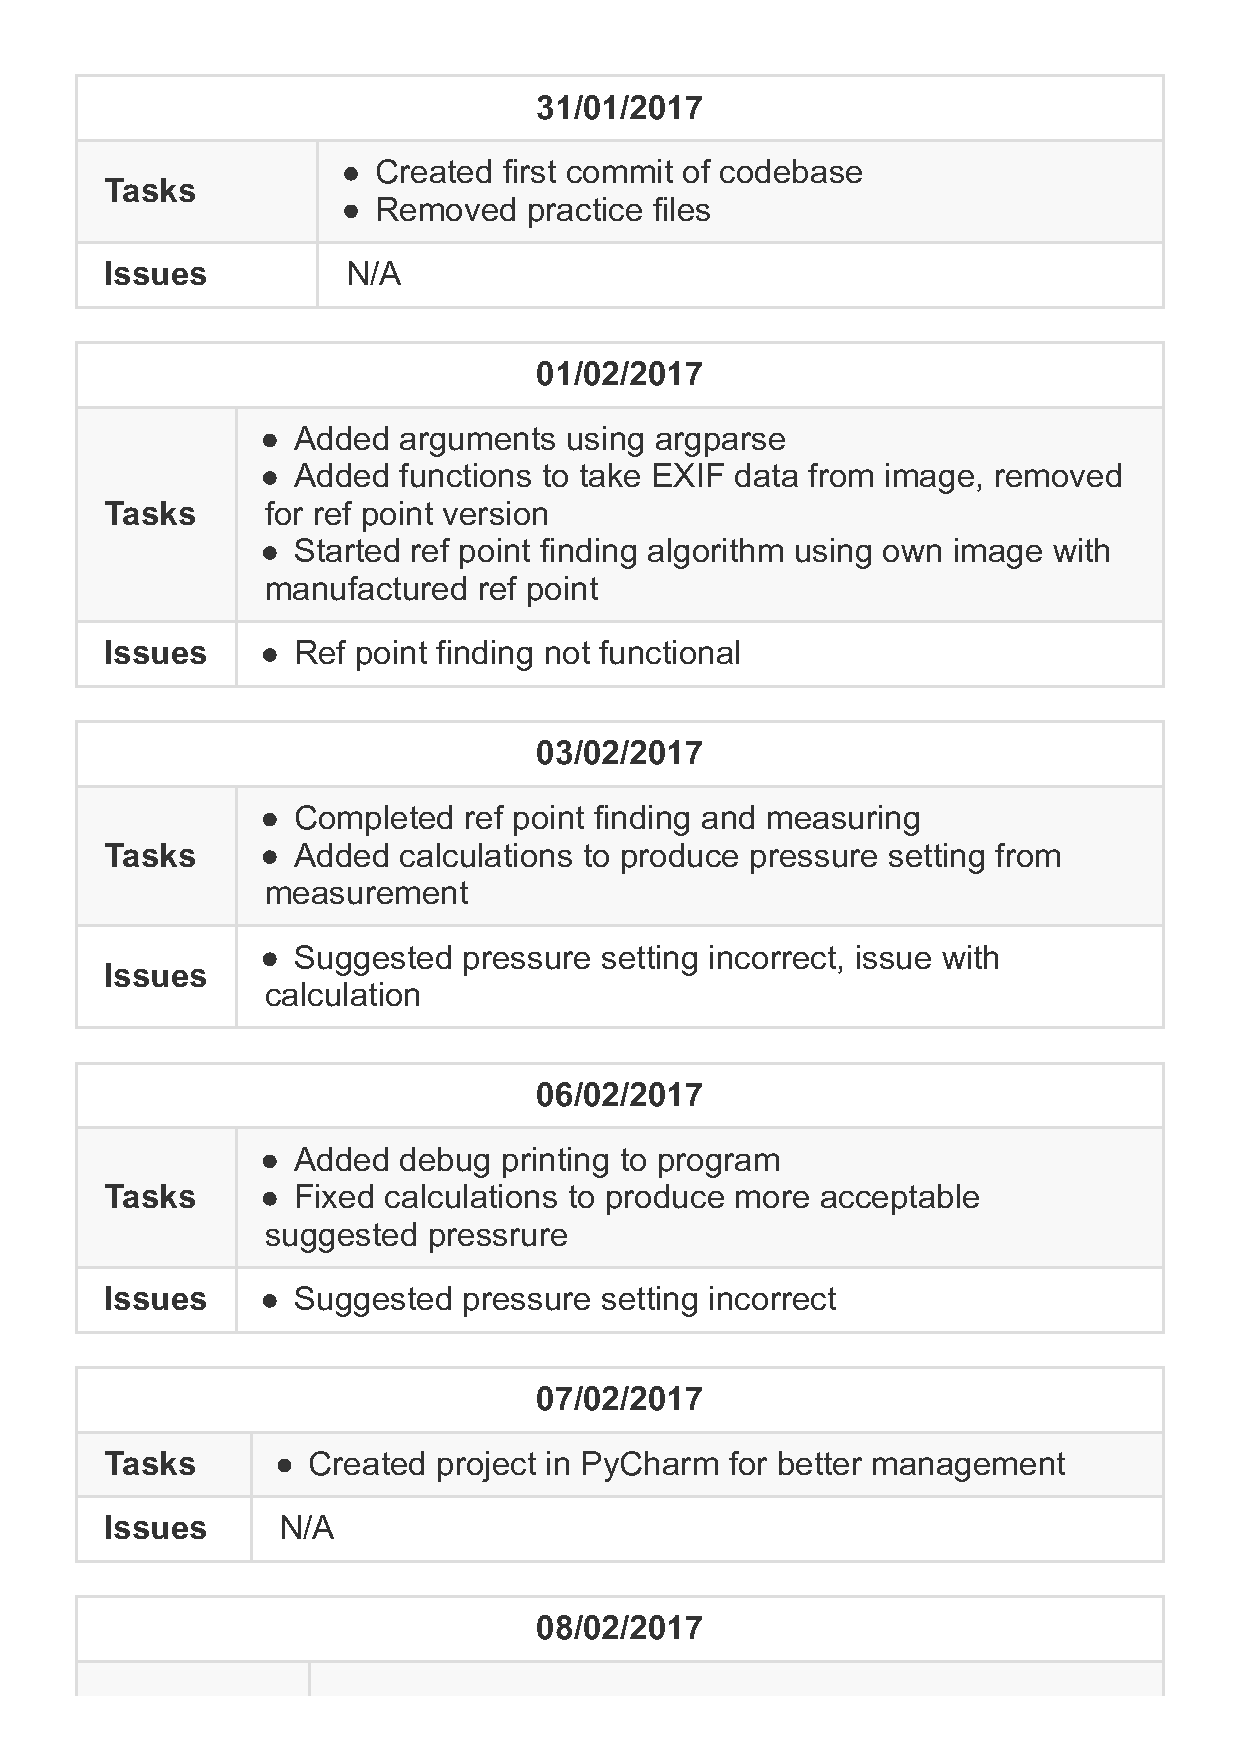
\includepdf[scale=0.8,
pages=1,
pagecommand=\section{Development Log}\label{app:dev_log}]
{../dev_log.pdf}
\includepdf[scale=0.8,
pages=2-]{../dev_log.pdf}
\clearpage
\section{Git Commit Log}\label{app:commit_log}
\inputminted[breaklines=true]{text}{../git_log.txt}
\clearpage
\section{Gantt Charts}\label{app:gantts}
	\subsection{Original}
		\begin{figure}[h!]
			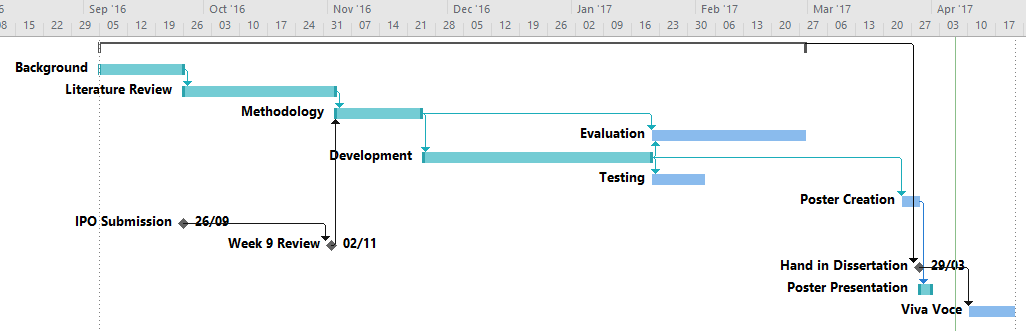
\includegraphics[width=\textwidth]{../images/gantt/orig/gantt.PNG}
		\end{figure}
		\begin{figure}[h!]
			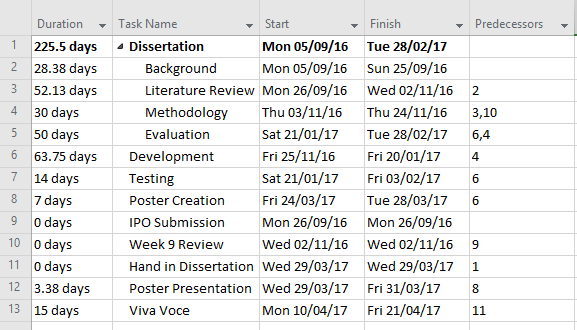
\includegraphics[]{../images/gantt/orig/tasks.PNG}
		\end{figure}
	\clearpage
	\subsection{First Revision}
		\begin{figure}[h!]
			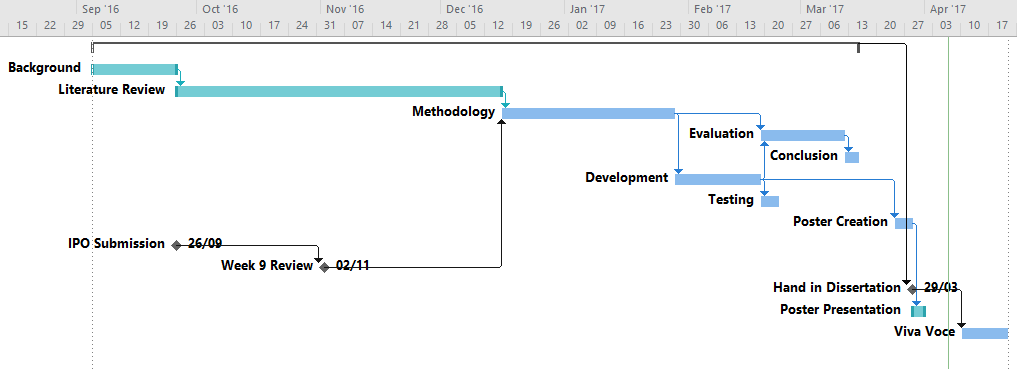
\includegraphics[width=\textwidth]{../images/gantt/v1/gantt.PNG}
		\end{figure}
		\begin{figure}[h!]
			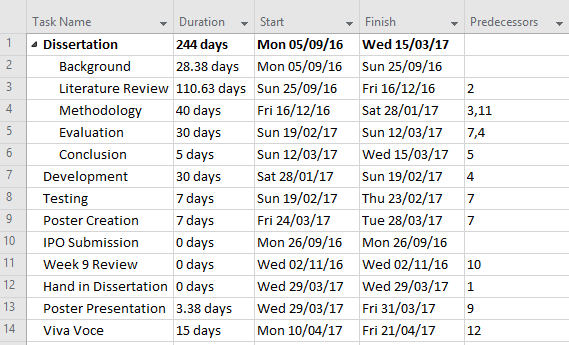
\includegraphics[]{../images/gantt/v1/tasks.PNG}
		\end{figure}
	\clearpage
	\subsection{Second Revision}
		\begin{figure}[h!]
			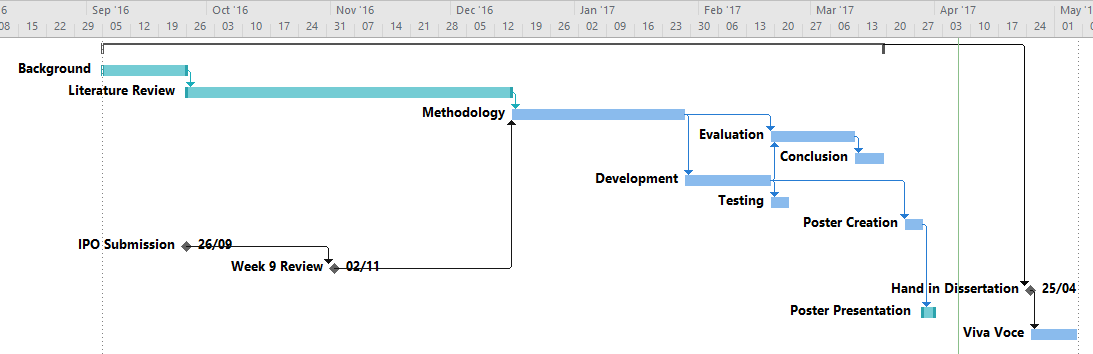
\includegraphics[width=\textwidth]{../images/gantt/v2/gantt.PNG}
		\end{figure}
		\begin{figure}[h!]
			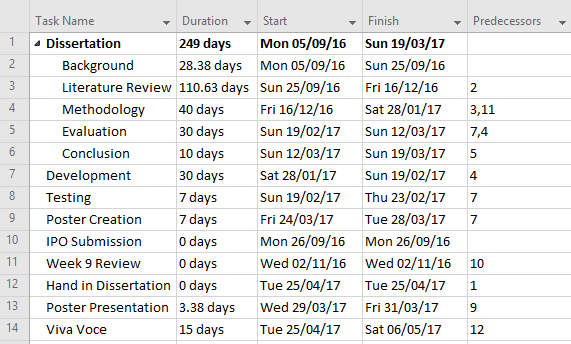
\includegraphics[]{../images/gantt/v2/tasks.PNG}
		\end{figure}
	\clearpage
	\subsection{Third Revision}
		\begin{figure}[h!]
			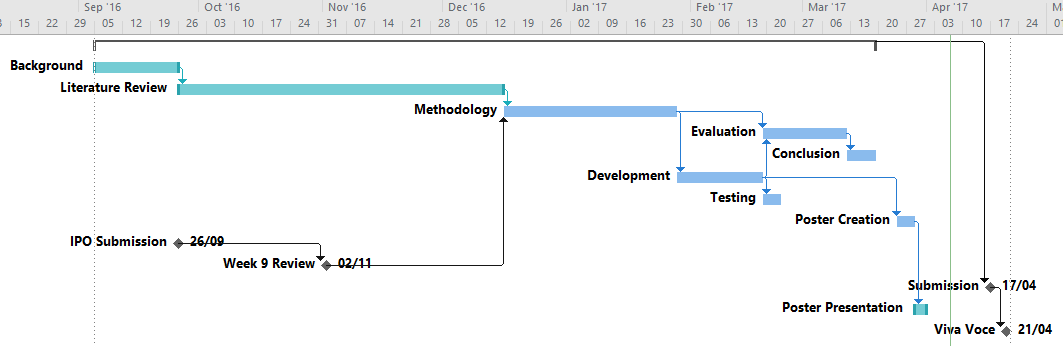
\includegraphics[width=\textwidth]{../images/gantt/v3/gantt.PNG}
		\end{figure}
		\begin{figure}[h!]
			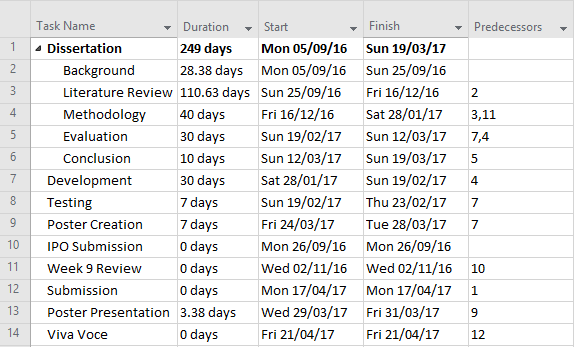
\includegraphics[]{../images/gantt/v3/tasks.PNG}
		\end{figure}
\clearpage
\section{Source Code}
	\subsection{main.py}
		\inputminted[breaklines,
					linenos,
					frame=lines,
					fontsize=\footnotesize]{python}{../code/final_program/main.py}
	\subsection{image\_processor.py}
		\inputminted[breaklines,
					linenos,
					frame=lines,
					fontsize=\footnotesize]{python}{../code/final_program/image_processor.py}
	\subsection{pressure\_calculator.py}
		\inputminted[breaklines,
					linenos,
					frame=lines,
					fontsize=\footnotesize]{python}{../code/final_program/pressure_calculator.py}
	\subsection{test\_image\_processor.py}
		\inputminted[breaklines,
					linenos,
					frame=lines,
					fontsize=\footnotesize]{python}{../code/final_program/test_image_processor.py}
	\subsection{test\_pressure\_calculator.py}
		\inputminted[breaklines,
					linenos,
					frame=lines,
					fontsize=\footnotesize]{python}{../code/final_program/test_pressure_calculator.py}